\section{The Prototype System}\label{sec:framework}
%In essence, our system is to reorganize the search log according to the structure of concepts and use the reorganized
%structure to quickly retrieve the matching historical queries and return them to user.
%
%In order to achieve that, we divide our system into two parts. One is the offline part, responsible for precomputing the
%index of search log. The other one is the online part, which can retrieve the index, rank the candidate queries and show
% results. As is shown in Fig. \ref{fig:overall-structure}, the two part is connected by the index of search log.

Our system is divided into two parts, an offline part which creates an index on
all historical search queries from the search log and an online runtime system
which retrieves a number of relevant queries to an input concept-based query
and ranks them according to a scoring function. The architecture of the system
is shown in Figure \ref{fig:overall-structure}.
%\KZ{Redraw this pic. Reposition
%the components to make it compact. Put offline part in dotted box and
%indicate so; put online part in dotted box and indicate so as well.}
Next, we briefly discuss the two key components in the architecture.

%Given a query, our system suggests user with more specific queries from search log
%according to relevance and quality. To do that, our system consists of two parts -- preprocessing
%part and runtime part. Preprocessing part conceptualizes each queries in search log and
%indexes them according to their concepts. Runtime part receives query from users and gives
%back a ranked list of suggestion queries with the help of index. As is shown in
%Fig. \ref{fig:overall-structure}, the two part is connected by the index of search log.
%
\begin{figure} [th]
  \centering
  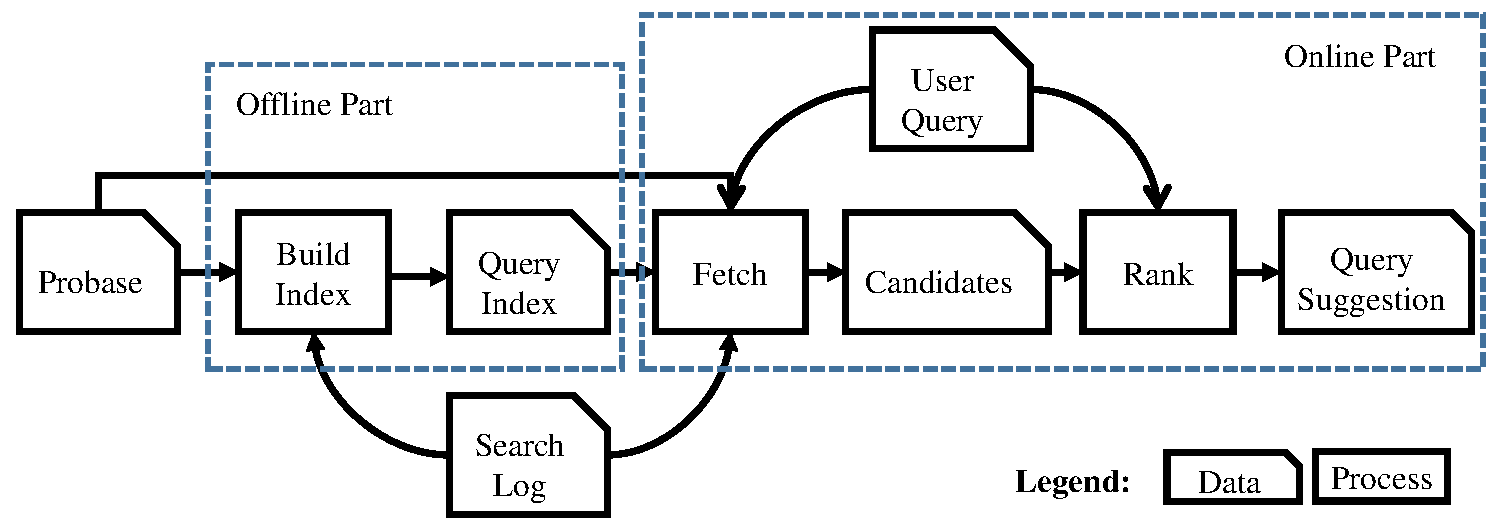
\includegraphics[width=0.8\columnwidth]{images/architecture}
  \caption{Architecture of System}
  \label{fig:overall-structure}
\end{figure}

\subsection{Build Index}\label{sec:index}
%In this step, our goal is to build an offline data structure according to the taxonomy of Probase \cite{wu2012probase},
%so that the runtime system can quickly find queries containing wanted concepts. The reprocessing step is performed in
%two steps.
First, we parse each historical query in the search log and identify
all noun-phrase terms which exist as entities in Probase.
Entities are those terms which appear
as the instance in at least one is-a pair in the taxonomy,
e.g., {\em katrina}, {\em louisina}, etc.
Then, we conceptualize these instances into their most likely concepts by
considering the neighboring instances in the same query, using the technique
by Song et al.\cite{Song11:Conceptualize,wang2012concept}.
For example, query ``{\em katrina} victims from {\em texas}''
maybe conceptualized into
``[hurricane] victims from [state]''. Finally, we build an index of
the search log using the concepts as keys.

%the historical queries according to their \textit{Probase instances} with the help of \textit{typicality} value.
%Secondly, we build an index according to the concepts of historical queries.

\subsection{Rank Candidates}\label{sec:rank}
%Fig. \ref{fig:runsys} shows a basic flow chart of runtime system. After loading needed data, it waits users for a query to process.
Given a query, our system first parses the query and recognizes the concepts
in it and then fetch a number of historical queries which are indexed by
these concepts as candidate suggestions.
%will refer to preprocessed index for related queries. Finally, the ranker is in charge of ranking the fetched
%historical queries and determines which queries should be returned to user. The key parts of our system are
%the parser and ranker.
%\begin{figure}
%  \centering
%  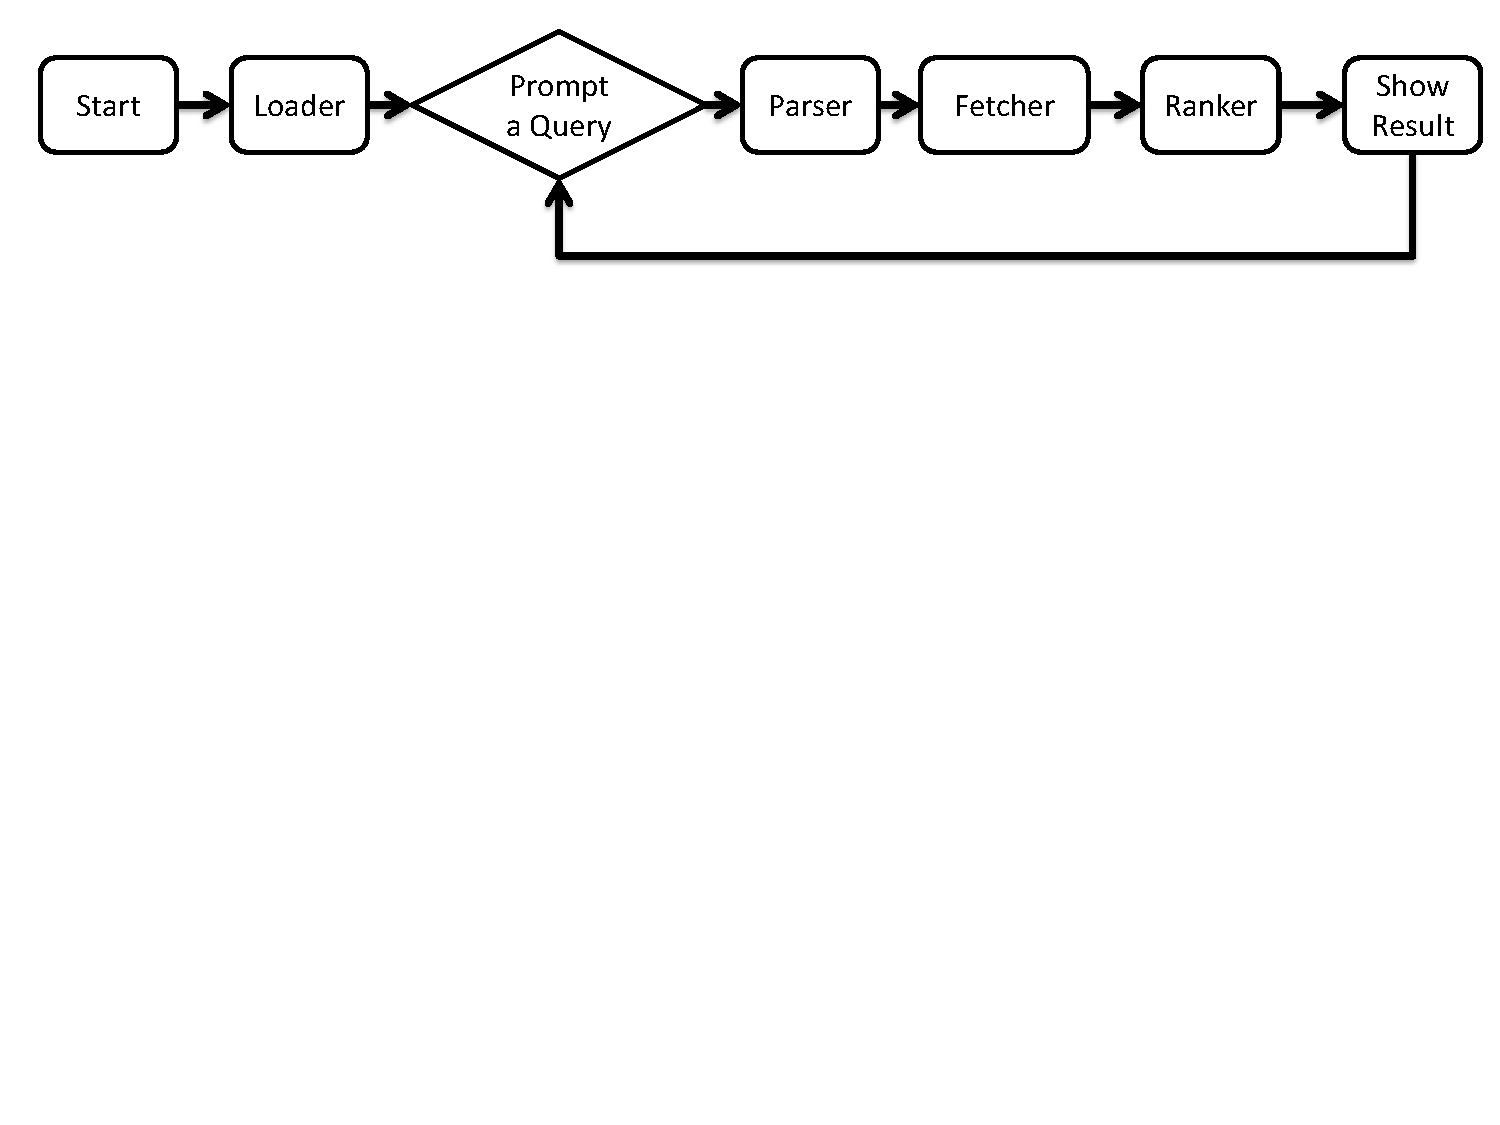
\includegraphics[scale=0.4]{images/system}
%  \caption{Overall Structure of Runtime System}
%  \label{fig:runsys}
%\end{figure}
%In the parsing stage, we firstly parse the input query with
%Stanford Parser \cite{klein2003accurate} and
%recognize all vague terms (i.e. \textit{Probase concept} here) in it
%and pass them to next stage. When recognizing concepts, our algorithm is kind of a greedy one,
%%as is shown in Algorithm \ref{alg:parse},
%which applies the strategy of left-to-right, maximum matching.
%
%\begin{algorithm}
%\caption{Parsing Function}
%\label{alg:parse}
%\begin{algorithmic} [1]
%  \REQUIRE a query Q;
%  \ENSURE a sequence of concepts and keywords SEQ;
%
%  \STATE $SEQ \Leftarrow PostagParser(Q)$ \\
%  \COMMENT {use a postag parser to do word-splitting and postaging}
%  \STATE $L \Leftarrow LengthOf(SEQ)$
%  \FOR {$max = L$ to $1$}
%    \FOR {$i = 0$ to $L - max$}
%      \IF {no concept from $SEQ[i]$ to $SEQ[i+max]$}
%        \STATE $Test \Leftarrow$ Link $SEQ[i]$ to $SEQ[i+max]$
%      \ENDIF
%      \IF {$Test$ is a concept}
%        \STATE $SEQ[i] \Leftarrow Test$
%        \STATE Mark $SEQ[i]$ as a concept
%        \STATE Remove $SEQ[i+1]$ to $SEQ[i+max]$
%        \STATE $L \Leftarrow L - max + 1$
%      \ENDIF
%    \ENDFOR
%  \ENDFOR
%  \RETURN $SEQ$
%\end{algorithmic}
%\end{algorithm}
Ranking the candidate is the main challenge in this work.
We apply a hybrid method to calculate the ranking score.
This score takes three factors into consideration,
i.e. semantic similarity, context similarity and quality of suggestion query.

The context similarity, $CScore$, is measured by the \textit{edit distance} between
the input query and the candidate in terms of
the number of insertion, deletion or replacement of words. Matched instances in
the candidate and the matched concepts in the input queries which
represent semantic information are removed before
calculating the edit distance.

The semantic similarity between a candidate query and an input query is the
combined distance between the instances in the candidate and the corresponding
concept in the input. The distance between an instance and a concept is
measured by the \textit{typicality} score between these two terms in
Probase. Because \textit{typicality} score is a value between 0 and 1 and can be
dense in some range (around 0.01 in practice), we take
logistic function on the typical value to expand the range into something
more distinguishable. We also use a scalar to make it linear  comparable with
$CScore$ according to statistics. That is,
\[SScore(t)=\beta \times (-\frac {1} {1+e^{-\alpha \times t}} + 1) \]
where $t$ is the \textit{typicality} value and $\alpha$ is the factor to
locate the dense range and $\beta$ is a scalar factor. Both factors are
learned from some training examples.
%\KZ{What is the key range?}

%The original version of \textit{Levenshtein distance} is described as the minimal edit distance
%from string to string by the unit of character. In order to underline the semantic meaning
%of queries, our modified version takes word as the basic unit in the algorithm.

We also utilize the click-through rate from the search log,
in order to measure the quality or effectiveness of candidate suggestion.
In this paper, we use a simple measure defined as
\[QScore(q)=\frac {\rm{Num\_clicks}(q)} {\rm{Frequency}(q)}\] 
where $q$ is a candidate suggestion query.
Besides the click-through rate, the quality score can be extended to
include other information from search log.

Currently, the overall score (the lower, the better) is defined as:
\[OverallScore = [CScore + SScore] + e^{-QScore} \]
%$QScore$ will be the determinant when $OverallScore$ is very close.

%\KZ{What's the definition of the overall score? Give the formula here.}
